\section{Experiments and Results}
\subsection{Reproducing Results}
\begin{figure}
    \centering
    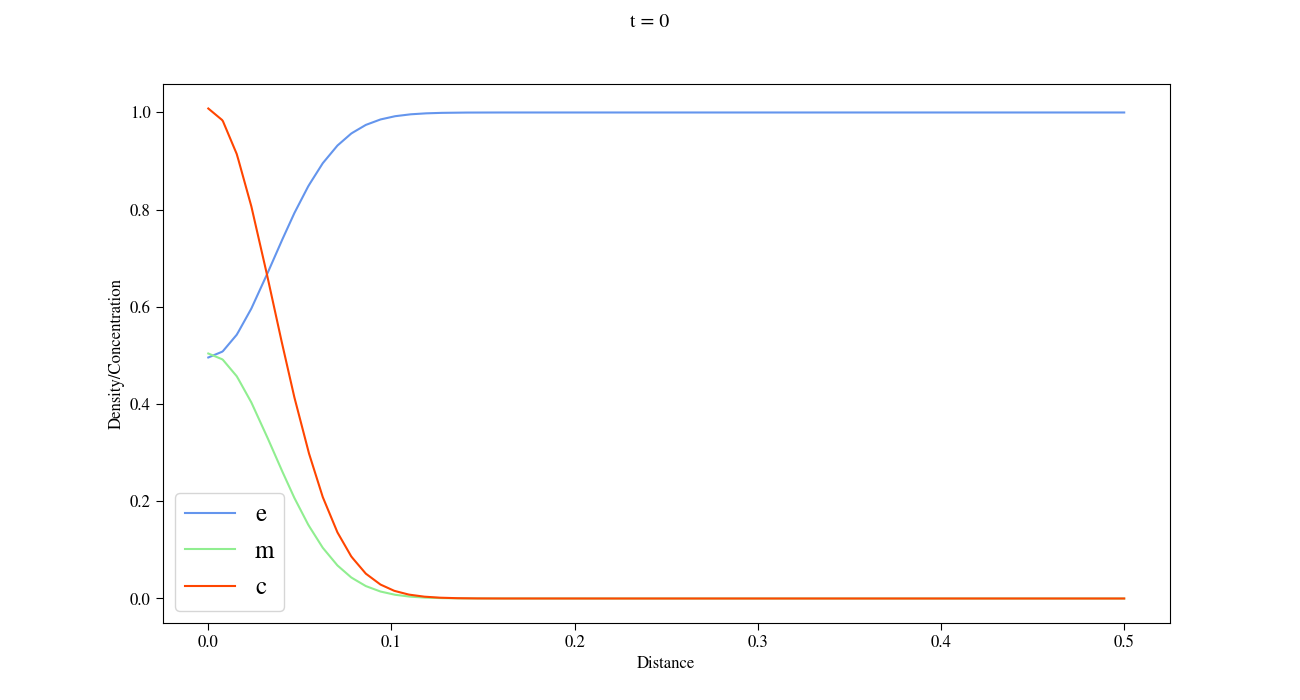
\includegraphics[width=\textwidth]{resources/images/inital_value_plot_figure.png}
    \caption{Caption}
    \label{fig:gliederung}
\end{figure}
\begin{figure}
    \centering
    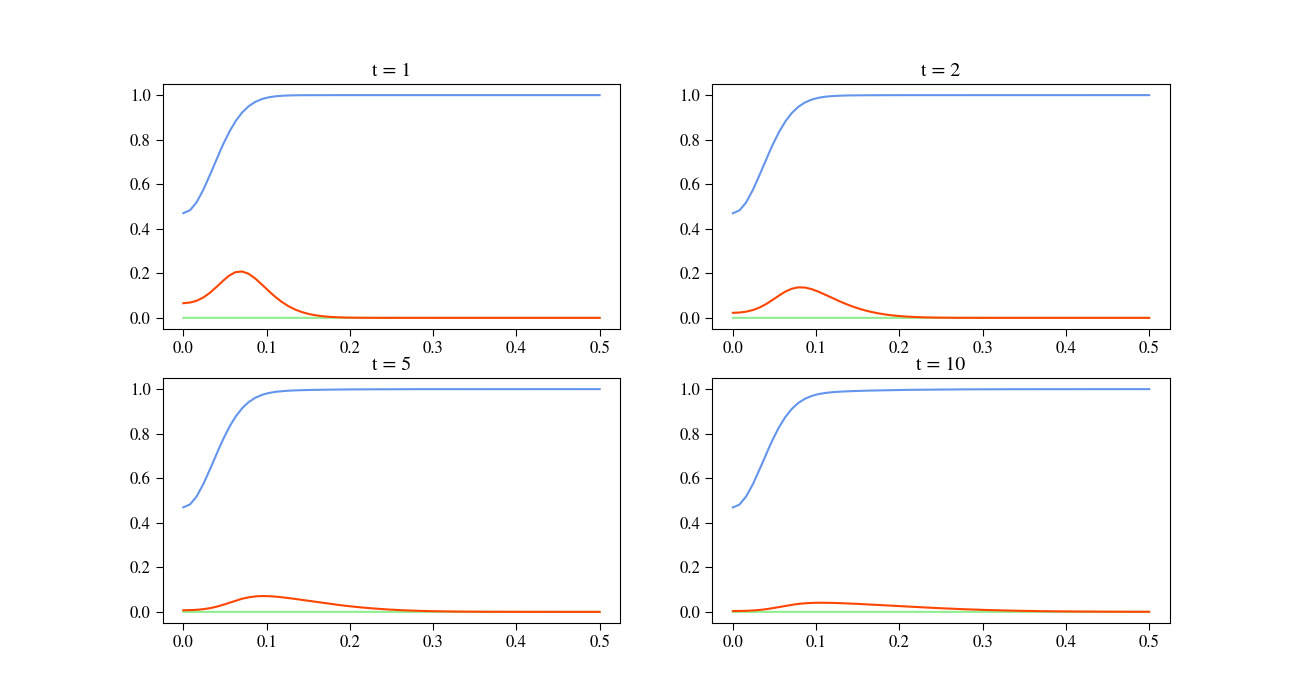
\includegraphics[width=\textwidth]{resources/images/0.001_0.001_0.001_10_0.1_0.5_0.005_0_0.png}
    \caption{Caption}
    \label{fig:gliederung}
\end{figure}
\begin{figure}
    \centering
    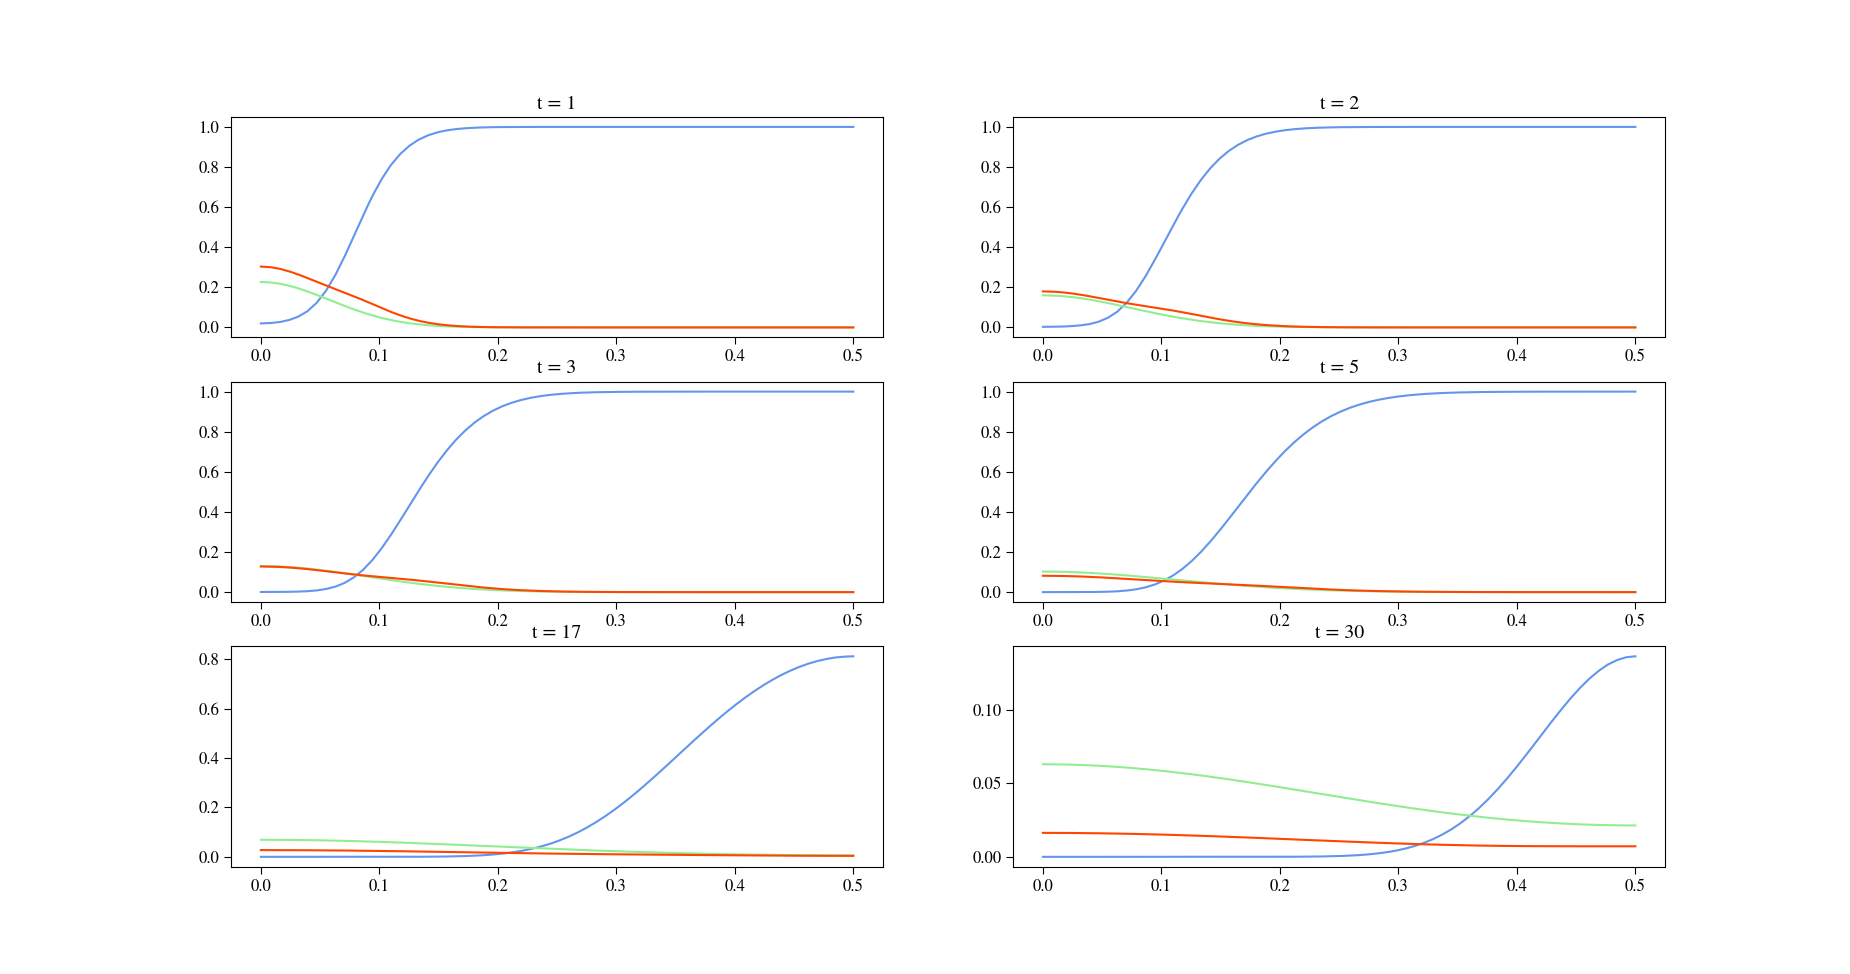
\includegraphics[width=\textwidth]{resources/images/0.001_0.001_0.001_10_0.1_0_0.001_0_0.png}
    \caption{Caption}
    \label{fig:gliederung}
\end{figure}
\begin{figure}
    \centering
    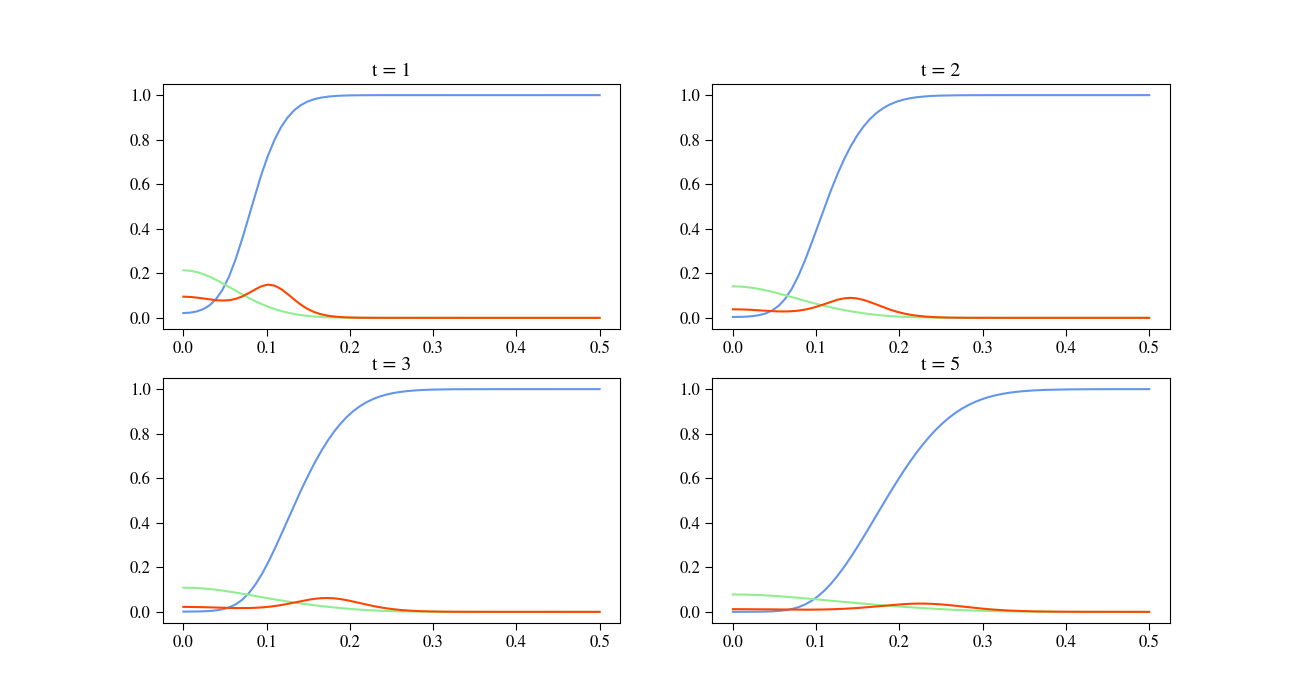
\includegraphics[width=\textwidth]{resources/images/0.001_0.001_0.001_10_0.1_0_0.005_0_0.png}
    \caption{Caption}
    \label{fig:gliederung}
\end{figure}
\begin{figure}
    \centering
    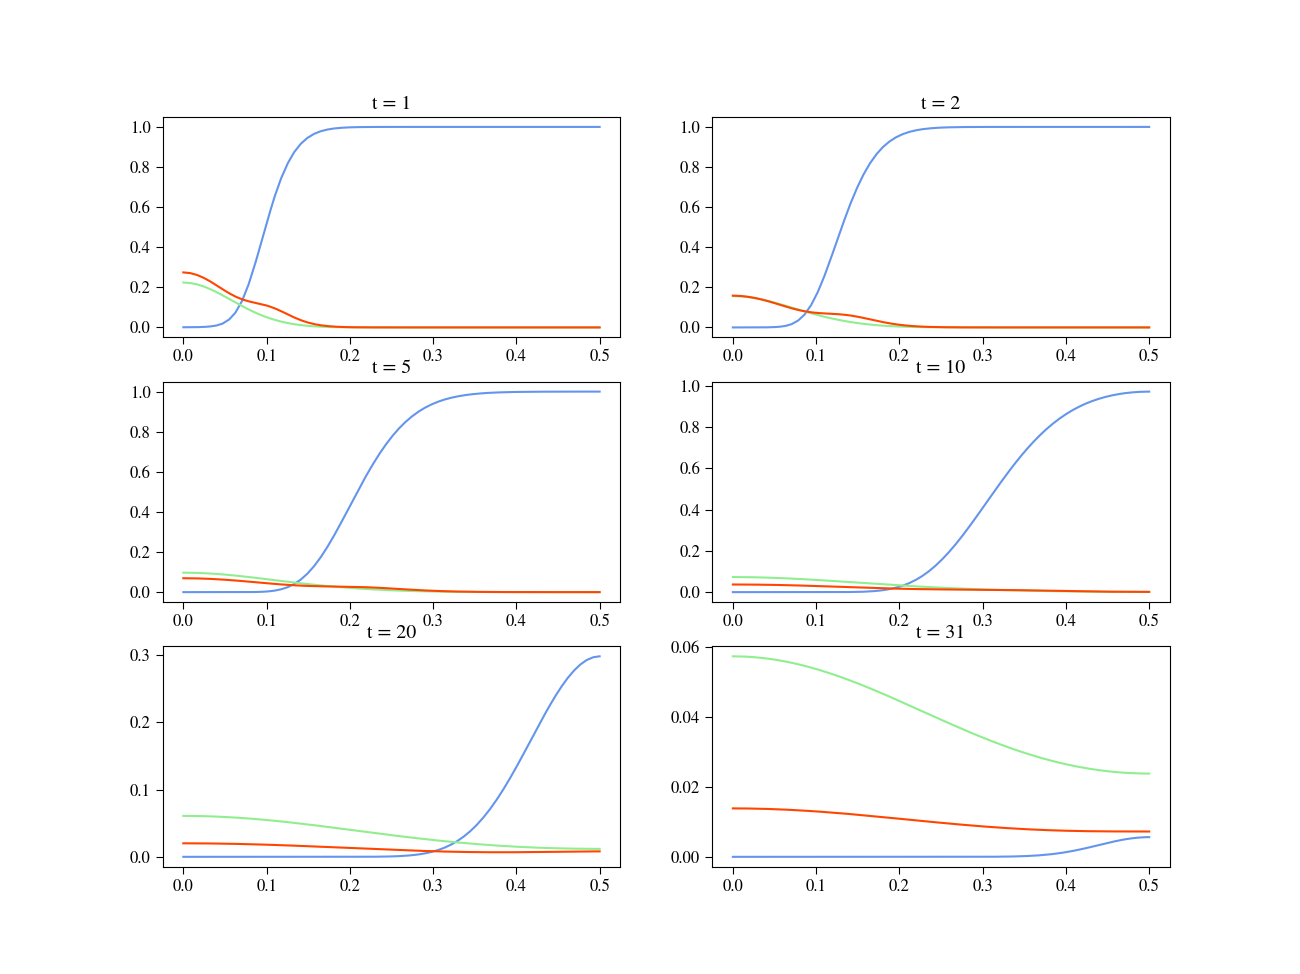
\includegraphics[width=\textwidth]{resources/images/0.001_0.001_0.001_20_0.1_0_0.002_0_0.png}
    \caption{Caption}
    \label{fig:gliederung}
\end{figure}
\subsection{2D Parameter Analysis}
\subsection{3D Parameter Analysis}
\subsection{3D Simulations with heterogenous ECM structure}